\documentclass[conference]{IEEEtran}
\usepackage{cite}
\usepackage{amsmath,amssymb,amsfonts}
\usepackage{graphicx}
\usepackage{textcomp}
\usepackage{xcolor}
\usepackage{booktabs}
\usepackage{tikz}
\usetikzlibrary{positioning,arrows.meta}
\usepackage[hidelinks]{hyperref}
\newcommand{\Fs}{F^{\star}}

\begin{document}

\title{Reached but Not Revealed: How Much Tests See at the Fix Site, and What It Means for Gemma~4 Coding Agents}

\author{\IEEEauthorblockN{Author Name}
\IEEEauthorblockA{\textit{Affiliation}\\
City, Country\\
email}}

\maketitle

\begin{abstract}
Coding agents are trained, selected and scored by running tests, so a test that runs a bug without failing is a blind spot in their reward. We trace which tests execute the code a reference fix edits (the fix site) and which fail, on the Gemma~4 Developer Agent dev set, eight libraries, and 104 SWE-rebench tasks from 96 independent repositories, all on CPU. Real bugs are reached but not revealed: in 77 of 78 SWE-rebench bugs, a median of 27 pre-existing tests executed the buggy function and none failed. Of 468 bugs planted at the fix site, the fail-to-pass tests catch 55\%, the full benchmark check 76\%, and no existing test 18\%. With the competition's own Gemma~4 31B checkpoint, candidates taken from runtime traces raise the model's correct first pick to 64\%, against 53\% from the provided code graph ($p=0.02$). A failing old test marks a Gemma patch as wrong 96\% of the time, but such tests miss 57\% of wrong patches. Adding these habits to a competition agent's prompt raised its dev-set resolve rate from 10.4\% to 15.6\% (106 tasks, two runs per arm; $p=0.026$). Agents should localize from runtime traces and test the behaviour the issue describes.
\end{abstract}

\begin{IEEEkeywords}
software testing, test oracles, coding agents, fault localization, Gemma, SWE-bench
\end{IEEEkeywords}

\section{Introduction}
An autonomous coding agent learns whether it succeeded from tests. Benchmarks such as SWE-bench~\cite{jimenez2024swebench} grade a patch by fail-to-pass (F2P) tests written for the issue and pass-to-pass (P2P) tests that must keep working; agents run the repository's tests to check themselves; reinforcement learning turns the same verdicts into reward. All three assume that a test which runs the relevant code would notice if that code were wrong.

Testing theory has long said otherwise. A fault is detected only if it is executed, infects the program state, propagates, and is revealed by an assertion~\cite{voas1992pie,ammann2016intro}. We ask how large the gap between \emph{reaching} and \emph{revealing} is in the places agents actually edit, and whether it changes what an agent should do. We measure it at the fix site~$\Fs$, the functions a task's reference fix edits, and test the consequences with Gemma~4 31B, the model the Gemma~4 Developer Agent competition requires.

Our contributions are:
\begin{itemize}
\item a CPU-only, per-test tracing pipeline that measures reach and reveal at $\Fs$, run on 4 competition repositories, 8 libraries and 96 independent SWE-rebench repositories;
\item a breakdown of who catches a fault at $\Fs$ (F2P, P2P, other existing tests, nobody), with confidence intervals;
\item two experiments with the competition's Gemma~4 checkpoint: which candidates to show the model when localizing, and how well old tests judge its patches;
\item concrete guidance for agents, tested as a paired dev-set A/B of a competition agent, plus a 2.7\,KB tracer agents can call.
\end{itemize}

\section{Background and Related Work}
\textbf{Reach, infection, propagation, reveal.} The PIE model~\cite{voas1992pie} and the RIPR conditions~\cite{ammann2016intro} separate executing a fault from detecting it. Pseudo-tested methods, whose bodies can be removed without any test failing~\cite{niedermayr2016will,vera2018descartes}, and checked coverage~\cite{schuler2011checked} show that coverage overstates what tests check. Coverage also correlates only weakly with suite effectiveness once suite size is controlled~\cite{inozemtseva2014coverage}. We measure the same gap at the fix site of benchmark tasks and on real agent patches.

\textbf{Mutants and real faults.} Mutants are a reasonable stand-in for real faults~\cite{just2014mutants,papadakis2018mutation}, but not a perfect one. We therefore report real bugs and real Gemma patches alongside planted ones.

\textbf{Fault localization.} Spectrum-based localization ranks code by how strongly failing tests execute it, for example with Ochiai~\cite{abreu2007accuracy}; PRFL diffuses such scores over a call graph with PageRank~\cite{zhang2017prfl}. We compare graph sources (runtime traces versus the static graph the competition provides) and test them with an LLM choosing among candidates.

\textbf{Benchmark tests are weak.} Patches that pass SWE-bench tests are often wrong~\cite{wang2026solved}; UTBoost~\cite{yu2025utboost}, SWE-ABS~\cite{yu2026sweabs} and program-variant probing~\cite{li2026probe} generate tests that expose them. Agentless filters patches with regression tests~\cite{xia2024agentless}. These works generate tests or rerank. We instead measure \emph{which existing test sets} observe the fix site, and how well old tests judge one model's patches.

\textbf{Non-normal dynamics.} Non-normal operators can amplify perturbations transiently even when every eigenvalue implies decay~\cite{trefethen2005spectra,asllani2018nonnormal}. We use this to quantify how far faults could spread through runtime call graphs.

\section{Method}
\begin{figure}[t]
\centering
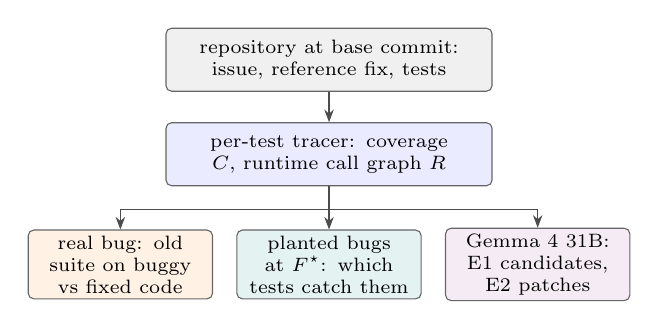
\begin{tikzpicture}[font=\scriptsize,
  box/.style={draw=black!60, rounded corners=2pt, align=center, inner sep=2pt, text width=#1, minimum height=8mm},
  arr/.style={-{Stealth[length=1.6mm]}, black!70}]
\node[box=40mm, fill=black!6] (in) at (0,0) {repository at base commit: issue, reference fix, tests};
\node[box=40mm, fill=blue!8] (tr) at (0,-1.2) {per-test tracer: coverage $C$, runtime call graph $R$};
\node[box=22mm, fill=orange!10] (real) at (-2.65,-2.6) {real bug: old suite on buggy vs fixed code};
\node[box=22mm, fill=teal!10] (mut) at (0,-2.6) {planted bugs at $\Fs$: which tests catch them};
\node[box=22mm, fill=violet!8] (gem) at (2.65,-2.6) {Gemma~4 31B: E1 candidates, E2 patches};
\draw[arr] (in) -- (tr);
\draw[arr] (tr.south) -- ++(0,-0.3) -| (real.north);
\draw[arr] (tr) -- (mut);
\draw[arr] (tr.south) -- ++(0,-0.3) -| (gem.north);
\end{tikzpicture}
\caption{Pipeline. One trace per task feeds three measurements: the response of the pre-existing suite to the real bug, which test sets catch bugs planted at the fix site~$\Fs$, and the context and grading for Gemma~4.}
\label{fig:pipeline}
\end{figure}

\textbf{Datasets.} Table~\ref{tab:data} lists the four datasets. The competition dev set has 129 tasks in four Python repositories (fastapi, rich, requests, httpx); 111 reproduce with their reference fix, and 101 can be traced. To test generality we use eight libraries (click, more-itertools, toolz, jinja, itsdangerous, packaging, marshmallow, boltons) at pinned releases, and SWE-rebench~\cite{badertdinov2025swerebench}. From SWE-rebench we draw 150 candidates (at most two per repository, Python 3.9--3.13, excluding the competition repositories); 104 build and reproduce, from 96 repositories. Everything runs on Kaggle CPUs except Gemma inference.

\begin{table}[t]
\caption{Datasets}
\label{tab:data}
\centering\scriptsize
\begin{tabular}{@{}lrrr@{}}
\toprule
Dataset & Repos & Tasks used & Planted bugs \\
\midrule
Competition dev set & 4 & 101 traced & 1,422 \\
Eight libraries & 8 & full suites & 339 \\
SWE-rebench (independent) & 96 & 104 of 150 & 468 \\
Gemma~4 E1 / E2 (dev set) & 4 & 96--99 / 88 & -- \\
\bottomrule
\end{tabular}
\end{table}

\textbf{Tracing.} A pytest plugin records, for every test, which package functions run, using \texttt{sys.monitoring} (Python~3.12+) or \texttt{sys.setprofile} with source-derived qualified names (3.9--3.11). This gives a test-by-function coverage matrix $C$ and a runtime call graph $R$ of observed caller--callee edges. Test outcomes are keyed by node id, so selection, tracing and grading use the same identifiers (98.5\% of selected tests matched in SWE-rebench mutant runs).

\textbf{Real bugs.} We run the pre-existing suite, without the task's test patch, on the buggy and the fixed code. A test \emph{reveals} the bug if it fails on the buggy code and passes on the fixed code. On SWE-rebench every such flip is re-run twice on each side and kept only if it is consistent.

\textbf{Planted bugs.} In the fixed code we plant single-site mutants in $\Fs$: comparison flips, Boolean operator swaps, negated conditions, constant changes and \texttt{return None}. For each mutant we run the tests that cover it (at most 300, sampled with a fixed seed) plus the F2P and P2P tests. A no-mutation control run flags unstable tests. We record whether the F2P tests, the full harness (F2P and P2P), or any covering test fails.

\textbf{Transient amplification.} For a runtime call graph $R$ with spectral radius $\rho$, let $M=R-(\rho+1)I$. Every mode of $e^{tM}$ decays, yet $A=\max_t\lVert e^{tM}\rVert_1$ can exceed~1 when $R$ is non-normal; $A=1$ for a normal matrix.

\textbf{Gemma~4.} We serve the competition's required checkpoint with vLLM~0.19.1~\cite{kwon2023vllm} on four L4 GPUs, offline and with thinking off (model \texttt{gemma-4-31b-it-\allowbreak qat-w4a16-ct}). In E1 the model sees the issue and 15 candidate functions in a seeded random order and names up to three to edit (greedy decoding). The candidates come from one of four sources: BM25 ranking of all functions against the issue text, failing-test coverage (Ochiai), coverage plus one hop on $R$, or coverage plus one hop on the competition's provided graph for that commit. In E2 the model gets the issue and the full source of $\Fs$, and returns rewritten functions: one greedy answer and four samples at temperature 0.8. Each distinct patch is graded by the \emph{harness} (all tests in the touched test files that pass with the reference fix) and by \emph{visible} tests: pre-existing tests, not added or edited by the test patch, that execute the edited functions and pass with the reference fix. An agent can run the visible tests itself.

\section{Reached but Not Revealed}
\textbf{Real bugs.} In the competition dev set the pre-existing suite executes $\Fs$ in 94 of 101 tasks, a median of 242 tests per task, and reveals the bug in one (93/94 silent). On SWE-rebench (Fig.~\ref{fig:real}) old tests execute $\Fs$ in 78 of 104 tasks (median 27, IQR 7--90). In 77 of those 78 (99\%; 95\% CI 96--100\%, resampling repositories), no old test fails on the bug and passes on the fix. The exception, in dandi-cli, is a genuine detection by nine tests. Silence is partly expected, since a shipped bug passed its project's CI. What the trace adds is that the suite \emph{ran} the buggy code, so the miss happened at reveal, not at reach.

\begin{figure}[t]
\centering
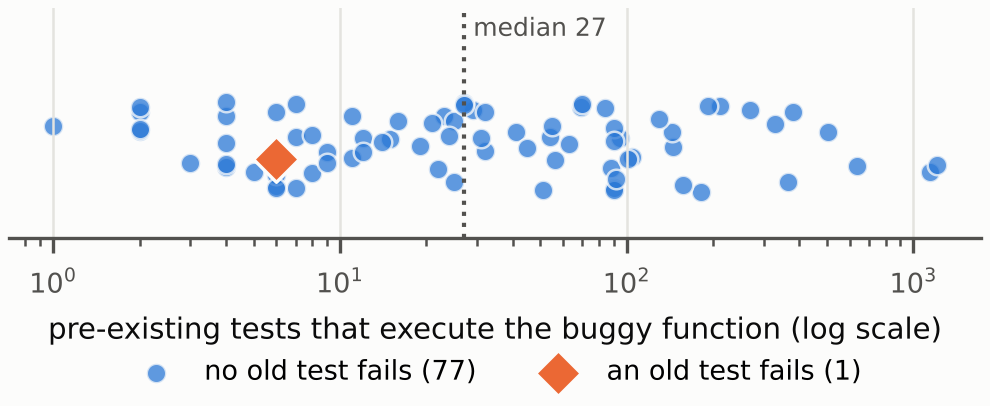
\includegraphics[width=\columnwidth]{figures/fig1_reach_not_reveal.png}
\caption{Real SWE-rebench bugs: for each task where old tests execute the buggy function, how many do. Only one task has an old test that fails on the bug and passes on the fix.}
\label{fig:real}
\end{figure}

\textbf{Planted bugs at the fix site.} On SWE-rebench, 468 bugs planted in $\Fs$ across 89 tasks split as in Fig.~\ref{fig:blind}. The task's F2P tests catch 55\% (95\% CI 48--62\%), P2P tests add 21 points, other existing tests add 6, and 18\% fail no existing test at all. The full benchmark check therefore accepts 24\% (18--31\%) of fix-site bugs. The F2P share is stable across datasets: 48\% on the competition dev set (where any covering test catches 81\%) and 51\% in a 30-task SWE-rebench pilot. Across all 1,422 competition mutants, 16\% of covered mutants make no test fail.

\begin{figure}[t]
\centering
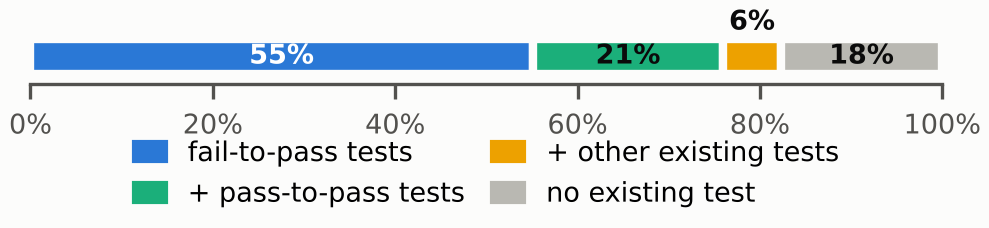
\includegraphics[width=\columnwidth]{figures/fig2_blind_spot.png}
\caption{Who catches a bug planted at the fix site (468 bugs, 89 SWE-rebench tasks; task-weighted). Segments are cumulative test sets.}
\label{fig:blind}
\end{figure}

\textbf{Spread is large, but does not predict detection.} Runtime call graphs are strongly non-normal. Transient amplification $A$ has a median of 5.1 on the competition repositories (maximum 28 for httpx, whose call graph is acyclic, so every eigenvalue is zero) and 3.7 on the eight libraries (range 2.0--14.7; 14.7 for itsdangerous, also acyclic). So faults \emph{could} spread far. Which tests notice, however, is governed by observation. The number of tests covering a mutated function predicts how many fail (Spearman $\approx$0.5--0.6). Graph-only measures (degree, Katz, PageRank, amplification) reach at most 0.35, and none adds information once coverage is known. Detection decayed only weakly with call depth on the competition repositories, and not at all within mutants in the libraries ($p=0.66$).

\textbf{Once a test fails, structure helps trace back.} Ranking functions by failing-test coverage (Ochiai) puts the fix in the top five in 30\% of competition tasks, and adding one hop on the runtime graph raises this to 53\%. On the same candidates, the runtime graph beats the competition's provided graph: 52\% versus 38\% top-5 and 28\% versus 11\% top-1 (90 tasks, $p=1.4\times10^{-6}$). On SWE-rebench, where the fix is usually one hop from what the failing test executes, the extra hop adds nothing (67\% to 71\%; 32 tasks better, 31 worse).

\section{Gemma~4 31B on the Dev Set}
\textbf{E1: which candidates to show the model.} Fig.~\ref{fig:e1} separates retrieval (is the fix among the 15 candidates?) from Gemma's choice (is its first pick the fix?). With runtime-trace candidates, Gemma's first pick is correct in 64\% of tasks (95\% CI 54--73\%). The provided graph gives 53\%, failing-test coverage alone 59\%, and issue text alone 43\%. In paired comparisons on the same tasks, runtime traces beat the provided graph in 13 tasks and lose in 3 ($p=0.02$, sign test), and beat issue-only retrieval 30 to 10 ($p=0.002$); both survive a Holm correction. The ordering holds in each of the two repositories that supply most tasks: 57\% versus 50\% in fastapi (55 tasks) and 72\% versus 56\% in rich (38). When the fix is among the candidates, Gemma picks it 74--91\% of the time, so retrieval is the bottleneck. The provided graph also lowers that conditional accuracy (74\% versus 81\% for runtime traces): its neighbours look plausible and distract the model.

\begin{figure}[t]
\centering
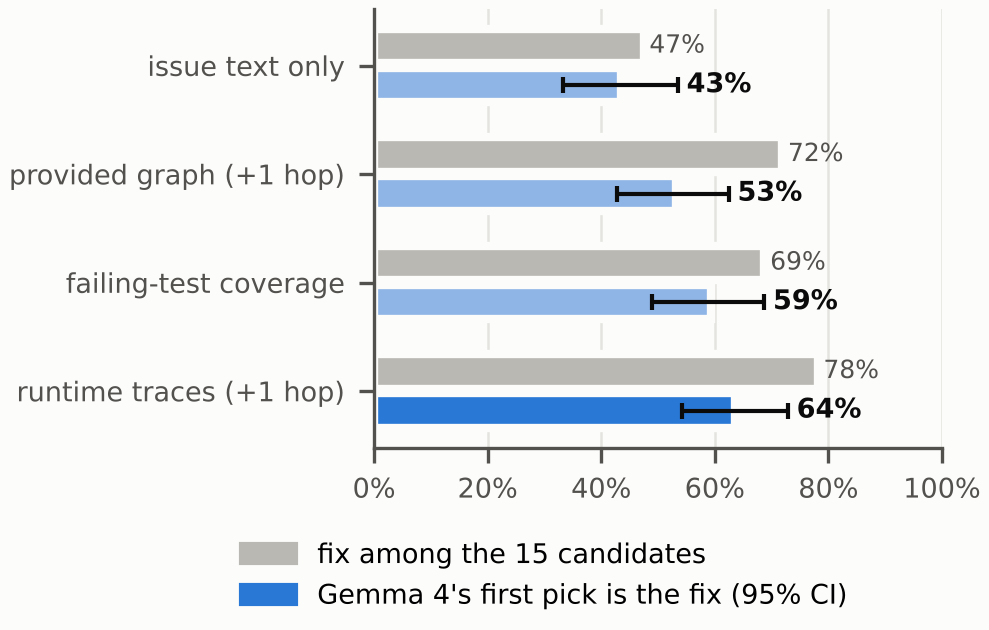
\includegraphics[width=\columnwidth]{figures/fig3_gemma_localization.png}
\caption{E1: Gemma~4 31B choosing the function to edit from 15 candidates whose source differs by condition (96--99 dev tasks). Grey: the fix is among the candidates. Blue: Gemma's first pick is the fix.}
\label{fig:e1}
\end{figure}

\textbf{E2: how well old tests judge Gemma's patches.} Over 88 tasks and 440 answers, 97\% are valid Python. The greedy answer resolves 38\% of tasks, sampled answers 41\%, and the best of five 45\%. Counting F2P tests only gives 39\%, so Gemma's failures are almost never ``broke something'': they are ``did not implement the new behaviour''. Visible tests exist in 94\% of tasks (median 90 per task). Fig.~\ref{fig:e2} compares the 212 wrong and 178 correct valid patches against them. A visible test fails for 43\% of wrong patches (95\% CI 31--56\%) and 2\% of correct ones. A flagged patch is therefore wrong 96\% of the time, while a patch that passes every visible test is correct only 59\% of the time. Choosing among the five answers by visible tests raises the resolve rate only from 38\% to 40\%, because answers disagreed in just 9 of 88 tasks.

\begin{figure}[t]
\centering
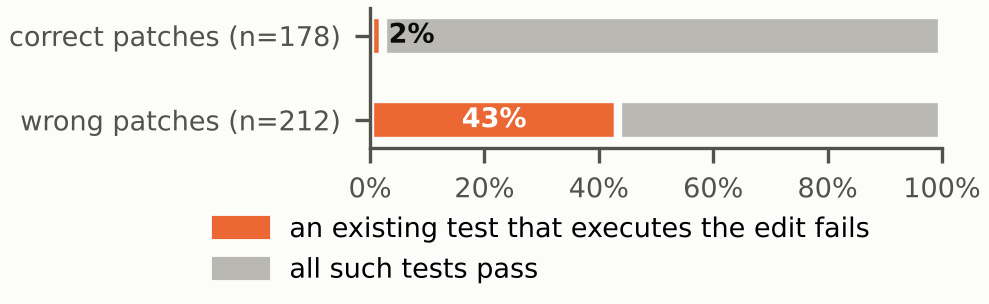
\includegraphics[width=\columnwidth]{figures/fig4_gemma_patches.png}
\caption{E2: Gemma~4 31B patches against pre-existing tests that execute the edit (88 dev tasks). Correctness is judged by the harness.}
\label{fig:e2}
\end{figure}

\section{Implications for Coding Agents}
The three results point the same way. An issue asks for behaviour the project's tests never asserted; otherwise the bug would not have shipped. The old suite therefore reaches the fix site without checking that behaviour, so it cannot reveal the bug and often cannot tell whether a fix worked. What it does check, it checks reliably, which is why a failing old test is such a strong signal. For agents this suggests three habits.
\begin{enumerate}
\item \emph{Localize from runtime traces.} Run the issue's reproduction under a tracer and show the model the functions the failing run executed, most suspicious first, not neighbours in a static graph (E1: 64\% versus 53\%).
\item \emph{Test the issue's behaviour directly.} More than half of wrong patches pass every old test (E2), so re-running the issue's example is the closest proxy for the hidden F2P tests.
\item \emph{Use old tests as a high-precision alarm.} A failing old test that executes the edit is a strong signal to retry (96\% precision), but a pass is weak evidence.
\end{enumerate}
\textbf{Dev-set A/B.} We added these habits to a competition agent by changing only its system prompt: the agent writes our 2.7\,KB tracer, localizes with it, checks the issue's example, and runs one regression check on the tests that execute its edit. We ran the original prompt (v2, 0.18 on the public leaderboard) and the new one (v3.2) twice each, with different sampling seeds, on the 106 dev tasks that reproduce. Both arms used the same model, a re-implementation of the competition's tools and limits (28 tool calls, 240\,s per command, and an 8-minute clock calibrated to single-stream speed), temperature 0.2 and thinking off. Patches were graded by the harness, using only tests that pass twice on the reference fix. Over both runs, v3.2 resolved 15.6\% of task runs (33 of 212) against 10.4\% for v2 (22 of 212), a gain of 5.2 points (95\% CI 1.4--9.4, bootstrap over tasks). v3.2 resolved more often on 14 tasks and v2 on 4 (task-level permutation $p=0.026$; sign test $p=0.031$), and each run alone favoured v3.2 (8 to 2 and 7 to 2). The gain comes from precision: when the agent edited, its patch was correct 60\% of the time with v3.2 (33 of 55) against 36\% with v2 (22 of 61), and wrong patches fell from 35 to 17. The cost is about 1.6 times more generated tokens. Both arms usually exhausted their 28 calls without editing (145 and 157 empty patches out of 212), so call budget, not verification, is now this agent's bottleneck.

For benchmark and reward designers, Fig.~\ref{fig:blind} is a budget. F2P tests alone leave about half of fix-site faults unobserved, adding P2P halves the remainder, and about a fifth needs new oracles, the gap that generated tests~\cite{yu2026sweabs,li2026probe} target.

\section{Limitations}
All measurements are on Python with pytest, and the tracer sees only Python-level calls. The Gemma experiments use the four dev-set repositories, greedy or lightly sampled decoding with thinking off, and oracle localization in E2, so absolute resolve rates are not leaderboard rates. The A/B uses our re-implementation of the tool interface rather than the official harness and two samples per arm; six v2 episodes lost their workspace and count as failures. Planted mutants are an imperfect proxy for real faults~\cite{just2014mutants}; we mitigate this with real bugs and real patches, which agree in direction. On SWE-rebench, 33 of 150 candidates failed reproduction, mostly because their F2P tests did not pass even with the fix, which points to environment drift. The SWE-rebench sample is drawn mostly from Python~3.9 tasks.

\section{Conclusion}
Across 108 repositories, tests reach the code agents edit far more often than they check it. Real bugs pass the suites that run them, a quarter of fix-site faults pass the full benchmark check, and more than half of Gemma~4's wrong patches pass every old test that runs them. The fix is not more graph structure but better observation. Agents should localize from what a failing run executes and test the behaviour the issue describes.

\section*{Data and Code Availability}
All notebooks (tracing, SWE-rebench, Gemma prompt pack, inference and grading, figures) and derived data (coverage matrices, call graphs, mutant outcomes, Gemma outputs) are on Kaggle: [link]. Every number in this paper is regenerated by the figures notebook.

\bibliographystyle{IEEEtran}
\begin{thebibliography}{99}
\bibitem{jimenez2024swebench} C.~E. Jimenez, J.~Yang, A.~Wettig, S.~Yao, K.~Pei, O.~Press, and K.~Narasimhan, ``SWE-bench: Can language models resolve real-world GitHub issues?'' in \emph{Proc. ICLR}, 2024.
\bibitem{voas1992pie} J.~M. Voas, ``PIE: A dynamic failure-based technique,'' \emph{IEEE Trans. Softw. Eng.}, vol.~18, no.~8, pp.~717--727, 1992.
\bibitem{ammann2016intro} P.~Ammann and J.~Offutt, \emph{Introduction to Software Testing}, 2nd~ed. Cambridge Univ. Press, 2016.
\bibitem{niedermayr2016will} R.~Niedermayr, E.~Juergens, and S.~Wagner, ``Will my tests tell me if I break this code?'' in \emph{Proc. Int. Workshop on Continuous Software Evolution and Delivery}, 2016.
\bibitem{vera2018descartes} O.~L. Vera-P\'erez, M.~Monperrus, and B.~Baudry, ``Descartes: A PITest engine to detect pseudo-tested methods,'' in \emph{Proc. ASE}, 2018.
\bibitem{schuler2011checked} D.~Schuler and A.~Zeller, ``Assessing oracle quality with checked coverage,'' in \emph{Proc. ICST}, 2011.
\bibitem{inozemtseva2014coverage} L.~Inozemtseva and R.~Holmes, ``Coverage is not strongly correlated with test suite effectiveness,'' in \emph{Proc. ICSE}, 2014.
\bibitem{just2014mutants} R.~Just, D.~Jalali, L.~Inozemtseva, M.~D. Ernst, R.~Holmes, and G.~Fraser, ``Are mutants a valid substitute for real faults in software testing?'' in \emph{Proc. FSE}, 2014.
\bibitem{papadakis2018mutation} M.~Papadakis, D.~Shin, S.~Yoo, and D.-H. Bae, ``Are mutation scores correlated with real fault detection?'' in \emph{Proc. ICSE}, 2018.
\bibitem{abreu2007accuracy} R.~Abreu, P.~Zoeteweij, and A.~J.~C. van~Gemund, ``On the accuracy of spectrum-based fault localization,'' in \emph{Proc. TAIC PART}, 2007.
\bibitem{zhang2017prfl} M.~Zhang, X.~Li, L.~Zhang, and S.~Khurshid, ``Boosting spectrum-based fault localization using PageRank,'' in \emph{Proc. ISSTA}, 2017.
\bibitem{wang2026solved} Y.~Wang, M.~Pradel, and Z.~Liu, ``Are `solved issues' in SWE-bench really solved correctly? An empirical study,'' in \emph{Proc. ICSE}, 2026.
\bibitem{yu2025utboost} B.~Yu \emph{et al.}, ``UTBoost: Rigorous evaluation of coding agents on SWE-bench,'' in \emph{Proc. ACL}, 2025.
\bibitem{yu2026sweabs} B.~Yu \emph{et al.}, ``SWE-ABS: Adversarial benchmark strengthening exposes inflated success rates on test-based benchmark,'' arXiv:2603.00520, 2026.
\bibitem{li2026probe} C.~Li, Y.~Xu, Z.~Wang, S.~H. Tan, and T.-H. Chen, ``Probe to generate: Program variant-guided test augmentation for repository-level repair benchmarks,'' arXiv:2604.01518, 2026.
\bibitem{xia2024agentless} C.~S. Xia, Y.~Deng, S.~Dunn, and L.~Zhang, ``Agentless: Demystifying LLM-based software engineering agents,'' arXiv:2407.01489, 2024.
\bibitem{trefethen2005spectra} L.~N. Trefethen and M.~Embree, \emph{Spectra and Pseudospectra: The Behavior of Nonnormal Matrices and Operators}. Princeton Univ. Press, 2005.
\bibitem{asllani2018nonnormal} M.~Asllani, R.~Lambiotte, and T.~Carletti, ``Structure and dynamical behavior of non-normal networks,'' \emph{Science Advances}, vol.~4, no.~12, 2018.
\bibitem{badertdinov2025swerebench} I.~Badertdinov \emph{et al.}, ``SWE-rebench: An automated pipeline for task collection and decontaminated evaluation of software engineering agents,'' arXiv:2505.20411, 2025.
\bibitem{kwon2023vllm} W.~Kwon \emph{et al.}, ``Efficient memory management for large language model serving with PagedAttention,'' in \emph{Proc. SOSP}, 2023.
\end{thebibliography}

\end{document}
